% !TEX root = main.tex

\section{The Framework: Reducing the Problem to a Multi-instance Collision Finder}\label{sec:setup}
Our task here is to upper-bound the advantage of an adversary in finding a short collision in a salted MD, according to the game $\gameG^{\aicr}_{N, M, B}$ described in Figure~\labelcref{fig:ex-game}. 
First, without loss of generality, in what follows, we assume that the adversary is deterministic. This follows since we can transform any probabilistic attacker into a deterministic one by hard-wiring the best randomness (see Adleman~\cite{SFCS:Adleman78}). 

We reduce the task of bounding the advantage of an attacker in finding a short collision in a salted MD, according to the game $\gameG^{\aicr}_{N,M,B}$, to a ``multi-instance'' game where the adversary does not have a preprocessing phase but instead only has a non-uniform auxiliary input, chosen \emph{before} the random oracle~$h$. The latter game is easier to analyze. 
Although the statement and reduction below were implicit in the work of Akshima et al.~\cite{AkshimaCDW20}, we make it formal and hopefully useful for future works. 


We define the following ``multi-instance'' game $\gameG^\uaicr_{N,M,B,u}(\sigma, \advA_2)$, where the preprocessing part of the adversary $\advA_1$ is degenerate and outputs the fixed string $\sigma$. More precisely, the game has the following steps: 
\begin{enumerate}
     \item $h \getsr \Func([N]\times [M], [N])$
    \item $U\getsr \binom{[N]}{u}$
    \item Define $\advA_1$ to be the algorithm that always outputs the string $\sigma$. 
    \item Return $\true$ if $\AICR_{h,a}(\advA = (\advA_1,\advA_2))=\true$ for every $a\in U$. Otherwise, return $\false$.
\end{enumerate}
For a string $\sigma$ and an adversary $\advA_2$, define
\begin{align*}
%\advA^{\uaicr}_{\MD,N,M,B}=\Prob{h\getsr \FuncNM, U\getsr \binom{[N]}{u}: (\forall a \in U : \AICR_{h,a}(\advA))}\;.  \\
\Adv^{\uaicr}_{\MD,N,M,B,u} (\sigma, \advA_2)=\Pr\left[ \gameG^\uaicr_{N,M,B,u}(\sigma, \advA_2) \right].
\end{align*}

\begin{lemma}%[Reducing to a multi-instance collision finder]
\label{lem:nu2ai}
Fix $N,M,B,S,T,u\in \mathbb{N}_{>0}$. Define $
\gamma :=  \left(\max_{\sigma,\advA_2} \left\{\Adv^{\uaicr}_{\MD,N,M,B,u} (\sigma, \advA_2) \right\}\right)^{\frac{1}{u}}$ where the maximum is taken over all $\sigma\in \{0,1\}^S$ and $T$-query algorithms $\advA_2$. Then, if $6N\gamma\geq u$,
\begin{align*}
\Adv_{\MD,N,M,B}^{\aicr}(S,T)  \le 6\cdot   \gamma + 2^{S-u},
\end{align*}
\end{lemma}
\newcommand{\lemmaone}{
\begin{proof}

\ifnum\eprintversion=0
\constructiveChernoffPrlims
\fi 

Define 
\begin{align*}
\gamma :=  \left(\max_{\sigma,\advA_2} \left\{\Adv^{\uaicr}_{\MD,N,M,B,u} (\sigma, \advA_2) \right\}\right)^{\frac{1}{u}}.
\end{align*}

We need to upper bound $\Pr_{h,a}\left[{\AICR_{h,a}(\advA)}=\true\right]$ for every $(S,T)$-AI adversary $\advA$. %Fix such $(S,T)$-AI adversary $\advA=(\advA_1,\advA_2)$.
We say that $h$ is \emph{easy} for adversary $\advA = (\advA_1,\advA_2)$ if $\advA$ wins the $\AICR_{h,a}$ game on a random $a\getsr[N]$ with probability $6\gamma$. That is, 
\begin{align*}
h \text{ is easy for } \advA \Longleftrightarrow \Pr_{a\getsr [N]}\left[\AICR_{h,a}(\advA) = \true\right]\geq 6\gamma .
\end{align*}

By the law of total probability, 
\begin{align*}
\Pr_{h,a}\left[{\AICR_{h,a}(\advA)}=\true\right] =& \Pr_{h,a}\left[{\AICR_{h,a}(\advA)=\true} \mid h\text{ is easy for }\advA\right]\cdot  \Pr_h[h\text{ is easy for }\advA] +\\&  \Pr_{h,a}\left[{\AICR_{h,a}(\advA) = \true} \mid h\text{ is not easy for }\advA\right]\cdot \Pr_h[h\text{ is not easy for }\advA] \\ 
\le & \Pr_h[h\text{ is easy for }\advA] + \Pr_{h,a}\left[{\AICR_{h,a}(\advA) = \true} \mid h\text{ is not easy for } \advA\right] \\ \le & \Pr_h[h\text{ is easy for }\advA] + 6\gamma.
\end{align*}
The lemma readily follows from the following claim where we prove an upper bound on $\Pr_h[h\text{ is easy for }\advA]$.
\begin{myclaim}
  Under the conditions of Lemma~\labelcref{lem:nu2ai}, for any $(S,T)$-AI adversary $\advA$, it holds that $\Pr_h[h\text{ is easy for }\advA] \le 2^{S-u}$.
\end{myclaim}
The proof of this claim follows simply by using the ``constructive Chernoff bound''~(Proposition~\labelcref{prop:chern}) and the union bound.
\begin{proof}
Fix an adversary as in the statement $\advA = (\advA_1,\advA_2)$. Define $\advA_\sigma$ the canonical preprocessing adversary that outputs the string $\sigma\in \{0,1\}^S$, ignoring its input. Denote $\advA_\sigma$ the $(S,T)$-AI adversary $(\advA_\sigma,\advA_2)$. By definition and by a union bound, it holds that  
\begin{align}
\Pr_h[ h\text{ is easy for }\advA ] &\le \Pr_h\left[ \exists \sigma\in \{0,1\}^S \colon h\text{ is easy for } \advA_\sigma \right] \nonumber\\
& \le 2^S \cdot \max_{\sigma\in \{0,1\}^S}  \Pr_h\left[h\text{ is easy for } \advA_\sigma \right].\label{eq:lemma1:unionbound}
\end{align}

For a fixed $a\in [N]$, $\sigma\in\{0,1\}^S$, and  $h \in \Func([N]\times [M],[N])$, define the indicator $X_{h,a}^\sigma=1$ if and only if $\AICR_{h,a}(\advA_\sigma) = \true$. By definition and with this notation,  for every $\sigma\in \{0,1\}^S$, it holds that
\begin{align}
\Pr_h\left[h\text{ is easy for } \advA_\sigma \right] & =   \Pr_{h}\left[\Pr_{a\getsr [N]} \left[\AICR_{h,a}(\advA_{{\sigma}}) =\true\right]   \geq 6\gamma\right] \nonumber\\&
   = \Pr_{h}\left[\Pr_{a\getsr [N]} \left[X^\sigma_{h,a}\right]\geq 6\gamma\right] \nonumber\\ 
  & = \Pr_{h}\left[\sum_{a\in [N]}X^\sigma_{h,a}\geq 6N\gamma\right].\label{eq:lemma1:sumbound}
\end{align}

By definition,  $\Adv^{\uaicr}_{\MD,N,M,B,u} (\sigma, \advA_2)$ is the advantage of the $T$-query attacker $\advA_2$ given auxiliary input $\sigma$ in finding collisions in salted MD relative to $h$ and on $u$ uniformly random salts denoted $U$. Written differently, for every $\sigma\in\{0,1\}^S$ and $T$ query adversary $\advA_2$, it holds that 
\begin{align*}
\Pr_{h,U}\left[\bigwedge_{a\in U}X_{h,a}^\sigma\right]&= \Adv^{\uaicr}_{\MD,N,M,B,u} (\sigma, \advA_2) \\ 
& \le \max_{\sigma^*,\advA_2^*} \left\{\Adv^{\uaicr}_{\MD,N,M,B,u} (\sigma^*, \advA^*_2) \right\}  = \gamma^u,
\end{align*}
where the last equality follows from the definition of $\gamma$.
Applying Proposition~\labelcref{prop:chern}, we get that for every $\sigma\in \{0,1\}^S$, it holds that 
\begin{align*}
\Pr_h\left[\sum_{a\in [N]}X^\sigma_{h,a}\geq 6N\gamma\right]\leq 2^{-u}.
\end{align*}

Plugging this back into~\eqref{eq:lemma1:sumbound}, we get that 
$\Pr_h\left[h\text{ is easy for } \advA_\sigma \right] \leq 2^{-u}$. In turn, plugging the latter back into~\eqref{eq:lemma1:unionbound}, we get that $\Pr_{h,a}\left[{\AICR_{h,a}(\advA)}=\true\right] \leq 2^{S-u}$, as needed.
\end{proof}
\end{proof}
}
\ifnum\eprintversion=1
\lemmaone
\else
The proof of this lemma is similar to a proof that appears in~\cite{AkshimaCDW20}. For completeness, we provide the full details in the full version~\cite{full}.
% Appendix~\labelcref{app:lemonepf}.
\fi
\section{Proving the STB Conjecture for $B\in O(1)$}\label{sec:comparg}
This section proves an upper bound on the advantage of any auxiliary-input adversary in the bounded-length collision resistance game of salted MD hash in the AI-ROM. The main theorem is stated next. 

\begin{theorem}\label{thm:MDST}
Let $C = \reqconst \cdot 6\cdot e^2$. For any $N,M,B,S,T\in \mathbb{N}_{>0}$ and fixing $\hat S := S + \log N$, it holds that 
\begin{align*}
  \Adv_{\MD,N,M,B}^{\aicr}(S,T) \leq \threshval+\frac{1}{N}\;.
\end{align*}
\end{theorem}

Theorem~\labelcref{thm:MDST} follows as a direct corollary of Lemma~\labelcref{lem:nu2ai} together with the following lemma and setting $u=S+\log N$.

\begin{lemma}[Hardness for a multi-instance collision finder] \label{lem:comp}
  Fix $N$, $M$, $B$, $S$, $T$, $u\in \mathbb{N}_{>0}$ and $\sigma\in \bits^S$. Then, for any $\advA_2$ that makes at most $T$ queries to its oracle for every salt, it holds that 
  \begin{align*}
  \Adv_{\MD,N,M,B,u}^{\uaicr}&(\sigma, \advA_2) \leq \\ & {\left(\uthreshval\right)}^u . 
    \end{align*}
\end{lemma}

The rest of this section is devoted to the proof of Lemma~\labelcref{lem:comp}. Unlike the proof of Lemma~\labelcref{lem:nu2ai}, the proof of this lemma is novel and differs completely from that of Akshima et al.~\cite{AkshimaCDW20}. The key conceptual insight is a structural characterization of collisions in $\MD_h$ that prevents the explosion in the number of cases that~\cite{AkshimaCDW20} faced during the case analysis.



% \subsection{Proof Overview of Lemma~\labelcref{lem:comp}}
%\subsection{Proof of Lemma~\labelcref{lem:comp}: Hardness for a multi-instance Collision Finder}\label{subsec:thm1:lemma2}
%



\subsubsection{Setup and notation} 



We are interested in bounding the advantage of the best strategy, i.e., a pair  $(\sigma,\advA_2)$ where $\sigma\in \{0,1\}^S$ is a fixed string and $\advA_2$ is a $T$-query algorithm, of finding bounded-length collisions in a salted MD with respect to the game $\gameG^\uaicr_{N,M,B,u}(\sigma, \advA_2)$.  Recall that in this game, $\advA_2$ needs to find proper collisions for $u$ randomly chosen salts, denoted $U$. The main idea in the proof is to use any such adversary  $(\sigma,\advA_2)$ to represent the function $h$ \emph{as well as} the set of random salts $U$ with as few bits as possible.  If the adversary is ``too good to be true,'' we will get an impossible representation, contradicting Proposition~\labelcref{complemma}.

\heading{Non-trivial range.} 
If either\begin{align*}
\frac{T^2}{N}>1\;\;\; \text{ or } \;\;\frac{uTB^2(3e\log u/\log\log u)^{2(B-2)}}{N}>1,
\end{align*}
 then Lemma~\labelcref{lem:comp} is trivially true. Hence, from now on we assume that both of the above left hand side terms are upper bounded by 1.

\paragraph{Setup.} Denote 
\begin{align*}
\zeta^* := {\left(\uthreshval\right)}^u.
\end{align*}
%
Assume the existence of an adversary $\advA = (\sigma,\advA_2)$, where $\sigma\in \{0,1\}^S$ is a string and $\advA_2$ is a $T$-query adversary, that contradict the inequality stated in the lemma. That is, there is $\zeta > \zeta^*$ such that
\begin{align}
\Adv_{\MD,N,M,B,u}^{\uaicr}(\advA)  := \zeta > \zeta^*. \label{eq:compression1}
\end{align}
 Define $\mathcal{G}$ to be the set of functions-sets of salts pairs for which the attacker succeeds in winning the game for every salt in the set relative to the function, That is, 
\begin{align*}
\mathcal{G}=\left\{(U,h) \,\middle\vert\, \MyAtop{U\in \binom{[N]}{u},}{h\in \FuncNM,} \forall a \in U:\AICR_{h,a}(\advA)=\true\right\}.
\end{align*}
%
Recall that $\zeta$ is defined to be the advantage of $\advA$ in the game $\gameG^\uaicr_{N,M,B,u}(\advA)$ in which $h$ and $U$ are chosen uniformly, and then $\advA$ needs to find a collision with respect to every one of the  $u$ salts in $U$. Therefore, 
\begin{align*}
| \mathcal G | = \zeta \cdot \binom{N}{u}\cdot N^{MN}.
\end{align*}
%If $\Adv^{\uaicr}_{\MD,N,M}=\epsilon$, it means that for exactly $\epsilon$ fraction of $(U,h)\in (\binom{[N]}{u} \times \FuncNM)$, $\forall a \in U:\AICR_{h,a}(\advA)=\true$. Therefore $|\mathcal{G}|=\epsilon\binom{N}{u}N^{MN}$.
In what follows we define an encoding and a decoding procedure such that the encoding procedure gets as input $U,h$ such that $U\in \binom{[N]}{u}$ and $h\in \FuncNM$, and it outputs an $L$ bit string, where $L = \log \left(\zeta^* \cdot \binom{N}{u}\cdot N^{MN}\right)$. The decoding procedure takes as input the string $L$ and outputs $U^*,h^*$. It will hold that $U^*=U$ and $h^* = h$ with probability $\zeta$.\footnote{Essentially, we will show that for all $(U,h)\in |\mathcal{G}|$, if the encoding procedure produces output $L$, then the decoding procedure on input $L$ outputs $U^*,h^*$ such that $U^*=U$ and $h^* = h$.}
Using Proposition~\labelcref{complemma}, this would give us that 
\begin{align*}
\log \zeta \le  L - \log \left(\binom{N}{u}\cdot N^{MN}\right) \Longrightarrow \zeta \le \zeta^*
\end{align*}
 which is a contradiction to the assumption (see~\eqref{eq:compression1}). 
 
%Using $\advA$, we shall define procedures $\Encode,\Decode$ such that for every $(U,h)\in \mathcal{G}$, $\Decode(\Encode(U,h))=(U,h)$ and the size of the output of $\Encode(U,h)$ is at most $L$ bits where $L=\log N^{MN}\binom{N}{u}(128e^2)^u\max\{\left(uT(3\log u/\log \log u)^{2(B-2)}B^2/N\right),\left(T^2/N\right)\}^u$.
%
%Using Proposition~\labelcref{prop:comp}, this would give us that 
%\[
%\epsilon\leq {\left(\uthreshval\right)}^u\;.  
%\]
%This immediately gives the bound claimed in the statement of the lemma. The rest of the proof of the lemma would define $\Encode,\Decode$, show an upper bound on the size of the output of $\Encode$ and that $\Decode(\Encode(U,h))=(U,h)$ for all $(U,h)\in \mathcal{G}$.



\heading{Notation and Definitions.} %Before giving the encoding and decoding procedures, we set up some notation and definitions.
%\heading{Fresh Salts.} 
To start off, we introduce some notations and definitions (we note that in Appendix~\labelcref{app:def} we summarize all the definitions we introduce in one place).
Fix $(U,h)\in \mathcal{G}$. Let $U=\{a_1,\ldots,a_u\}$ where the $a_i$'s are ordered  lexicographically. 
Let $\Queries(a)\in ([N]\times [M])^T$ be the list of queries that $\advA_2$ makes to $h$ when executed with input $({\sigma},a)$. Namely, for $a\in [N]$,
\begin{align*}
\Queries(a) = \left\{ (a',\alpha') \in [N]\times [M] \mid \advA_2(\sigma,a) \text{  queries $h$ on   $(a',\alpha')$}\right\}\;.
\end{align*}
Note that $\Queries(a)$ is indeed a set as we can assume (without loss of generality) that $\advA_2$ never repeats queries in a single execution (since $\advA_2$ can just store all of its past queries).

We say that $a'\in \Salts(a)$ if there is some $\alpha'\in [M]$ such that $(a',\alpha')$ is an entry in $\Queries(a)$. Namely, for $a,a'\in [N]$, 
\begin{align*}
a'\in \Salts(a) \Longleftrightarrow \exists \alpha' \in [M] \text{ s.t. } (a',\alpha') \in \Queries(a).
\end{align*}
 We define the set of \emph{fresh} salts in $U$. A salt $a_i$ for $i \in [u]$ is called fresh if it was never used as the salt in any query performed by $\advA_2$ while being executed on salts $a_j$ for $j\le i-1$ which are fresh. The first salt $a_1$ is always fresh. A salt $a_i$ for $i \ge 2$ is fresh if for any fresh $a_j$ for $j \le i-1$, $a_i \notin \Salts(a_j)$. Namely, denoting the set of fresh salts by $\uf$, we have the following inductive (on $i\in [u]$) definition:
 \begin{align*}
a_i\in \uf \Longleftrightarrow \forall j\le i-1,  a_j \in \uf\colon a_i \not \in \Salts(a_j).  
\end{align*}
Looking ahead, we define $\uf$ like this because we run $\advA_2$ on the salts in $\uf$ in lexicographical order, and this definition ensures that each salt that $\advA_2$ is executed on was not queried by it previously. Denote 
\begin{align*}
F := |\uf| \quad \text{ and }  \quad \uf=\{a_1',\ldots,a_F'\} \text{ (ordered lexicographically).}
\end{align*}
Denote
\begin{align*}
 \forall i\in [F]\colon \q_i:=\Queries(a_i') \quad \text{ and } \quad \qf:=\q_1\concat\ldots\concat \q_F,
 \end{align*}
 where $\concat$ is the concatenation operator. Let $\qf[r]$ be the $r$th query in the list $\qf$. Note that $r\in [F\cdot T]$.
 For every $a\in U\setminus \uf$, let $t_a$ be the minimum value such that $\qf[t_a]$ is a query with salt $a$. 
 Define the set of \emph{prediction} queries as 
 \begin{align*}
 \Pred:=\{t_a\mid a\in U\setminus \uf\}.
 \end{align*}
The encoding algorithm will output $\uf,\Pred$, along with a list of evaluations of $h$ (this list is determined by running $\advA_2$) which suffices to recover the set $U$ by running $\advA_2$ during decoding.

 We let $\hrest$ be the list of $h(a,\alpha)$ values when executed on distinct queries in $\qf$, in the same order as they appear in $\qf$, followed by the evaluation of $h$ on the following values in lexicographical order of the inputs. 
 \[
 \{(a,\alpha):a\in [N],\alpha\in [M]\}\setminus \qf\;.
 \]
 Therefore, $\hrest$ is initialized to contain the evaluation of $h$ at all points in its domain. Looking ahead, in the encoding procedure, we will remove elements from $\hrest$ as needed to compress $h$.


\heading{Function and Query graphs.} 
A notion that will be useful is that of a ``function graph''. 
\begin{definition}[Function graph]
For a function $h:[N]\times [M]\to [N]$, consider the following directed graph: it has $N$ nodes labelled with elements of $[N]$ and each node has exactly $M$ outgoing edges, each labelled with elements of $[M]$. There is an edge from node $a_i$ to $a_j$ labelled $\alpha$ if and only if $h(a_i,\alpha)=a_j$.
\end{definition}
\noindent We define the notion of query graph for an adversary as follows.
\begin{definition}[Query graph]
Execution of an adversary $\advA_2$ on salts $a_1',\ldots,a_F'$ defines a query graph as follows. Initially the graph is empty. Whenever  $\advA_2$ queries $(a,\alpha)$ to $h$, we add a node with label $a$ if not already present and add an edge $(a,h(a,\alpha))$ with label $\alpha$ if not already present.
\end{definition}
We explicitly note that the query graph evolves as the adversary keeps making queries. 
\begin{fact}
The query graph is always a sub-graph of the function graph of $h$.
\end{fact}
\heading{Structure of collisions: The mouse structure.}
Since adversary $\advA_2$ succeeds on all of the salts in $U$, it holds that for every $j\in [F]$, the output of the adversary is $(\alpha_j,\alpha_j')$ 
such that $\alpha_j\neq \alpha_j'$, $\MD_h(a_j',\alpha_j)=\MD_h(a_j',\alpha_j')$ and both $\alpha_j,\alpha_j'$ are at most $B$ blocks long.
We can assume without loss of generality that the colliding messages $\alpha_j$ and $\alpha_j'$ are ``minimal'' (because otherwise, we can trim $\alpha_j,\alpha_j'$ to obtain a shorter collision).
The evaluations of $h$ in order to compute $\MD_h(a_j',\alpha_j)$ and $\MD_h(a_j',\alpha_j')$ induce a structure that we call a \emph{mouse structure} as shown in Fig.~\labelcref{fig:mouse-structure}.
More explicitly, suppose the output of the $\advA_2$ is $(\alpha_j=(\alpha_{j,1},\ldots,\alpha_{j,B_1}),\alpha_j'=(\alpha_{j,1}',\ldots,\alpha_{j,B_2}'))$ for $B_1,B_2\leq B$ such that $\alpha_{j,i}=\alpha_{j,i}'$ for all $1 \leq i\leq k$ where $k\geq 0$. 
Define $(x_1,\ldots,x_k,y_1,\ldots,y_{k'},z_1,\ldots,z_{k''})$ where $k'=B_1-k,k''=B_2-k$ as follows. (If $k'=0$ then $y_i$'s are not defined, and if $k''=0$ then $z_i$'s are not defined.)
\begin{align*} 
  &x_1= h(a_j',\alpha_{j,1})\;,\; x_i=h(x_{i-1},\alpha_{j,i}) \text{  for $1< i\leq k$}\\
  &y_1= \begin{cases}
    h(a_j',\alpha_{j,1}) &\text{ if }k=0\\
    h(x_k,\alpha_{j,k+1})&\text{ otherwise}
  \end{cases}\;,\;
  y_i=h(y_{i-1},\alpha_{j,i+k}) \text{    for $1< i\leq B_1-k$}\\
  &z_1= \begin{cases}
    h(a_j',\alpha_{j,1}')&\text{ if }k=0\\
    h(x_k,\alpha_{j,k+1}')&\text{ otherwise}
  \end{cases}\;,\;
  z_i=h(z_{i-1},\alpha_{j,i+k}') \text{    for $1< i\leq B_2-k$}\\
\end{align*}
\begin{figure}
  \centering
  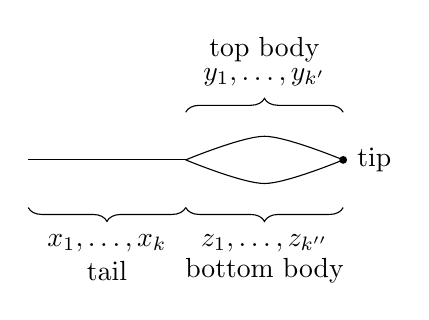
\begin{tikzpicture}
      \draw (-1,0) -- (1,0);
      % \node[circle,inner sep=1pt,fill=red,label=left:{salt}] at (0,0) {};% 
      \node[circle,inner sep=1pt,fill=black,label=right:{tip}] at (3,0) {};% 
      \draw [decorate,decoration={brace,amplitude=5pt,mirror,raise=4ex}]
    (1,0) -- (3,0) node[midway,yshift=-3em]{$z_1,\ldots,z_{k''}$} 
                        node[midway,yshift=-4em]{bottom body};
    \draw [decorate,decoration={brace,amplitude=5pt,mirror,raise=4ex}]
    (-1,0) -- (1,0) node[midway,yshift=-3em]{${x_1,\ldots,x_k}$}
                          node[midway,yshift=-4em]{tail};
    \draw [decorate,decoration={brace,amplitude=5pt,raise=4ex}]
    (1,0) -- (3,0) node[midway,yshift=3em]{$y_1,\ldots,y_{k'}$}
                        node[midway,yshift=4em]{top body};
      \draw plot[smooth] coordinates{(1,0) (2,0.3) (3,0)};
      \draw plot[smooth] coordinates{(1,0) (2,-0.3) (3,0)};
  \end{tikzpicture}
  \caption{A mouse structure. For ease of visual representation we do not draw the nodes and edges of the graph, instead represent it as a continuous structure.} \label{fig:mouse-structure}
  \end{figure}
Then $(x_1,\ldots,x_k,y_1,\ldots, y_{k'},z_1,\ldots,z_{k''})$ form a mouse structure as specified in Figure~\labelcref{fig:mouse-structure}. (If $k'=0$, the mouse structure is formed only by $x_1,\ldots,x_k,z_1,\ldots,z_{k''}$ and if $k''=0$, the mouse structure is formed only by $x_1,\ldots,x_k,y_1,\ldots,y_{k'}$).
Without loss of generality, we can assume that the mouse structure is present in the query graph of $\advA_2$ before it outputs the answer for salt $a_j'$.
We refer to this structure as the mouse structure for salt $a_j'$.
% If there are multiple such structures, we choose the shortest one, and if there is a tie, we choose one arbitrarily.  

  
We define $\uq_j$ to be the set of queries in the mouse structure. Similarly, we define  $\us_j$ as the set of salts that comprise the mouse structure. By definition, $1\leq |\uq_j|, |\us_j|\leq 2B$. 

\heading{Classifying queries.} We classify every one of the queries in $\qf$ into one of 3 types by scanning through them in order. Recall that $\qf$ consists of $F$ blocks, each consisting of $T$ queries. Each block contains a mouse structure as in Figure~\labelcref{fig:mouse-structure}.
The first type of query is called \new. A \new\ query did not appear in any previous block. Non-\new\ queries are called \emph{repeated} and they are classified further into one of 2 types: \frep, and \urep. A query $(a,\alpha)$ would be a \frep\ query if it was made as part of a mouse structure during some earlier salt in $\uf$. Lastly, a \urep\ query is one that was made before but is not part of any mouse structure. That is,
\begin{enumerate}
\item \new: A query with index $r\in [F\cdot T]$ is \new\ if there does not exist $r'<r$ such that $\qf[r']=\qf[r]$. 
\item A non-\new\ queries is called \emph{repeated}. We classify the latter into two subcategories:
\begin{enumerate}
\item \frep: 
A query in $\q_j$ with index $s\in [T]$ such that $h(\q_j[s])=a$ is \frep\ if it is not \new\ and $\q_j[s]\in \uq_i$ for some $i<j$.
\item \urep: A query in $\q_j$ with index $s\in [T]$ such that $h(\q_j[s])=a$ is  \urep\  if it is not \new, $\q_j[s]\not\in \uq_i$ for all $i<j$.
\end{enumerate}
\end{enumerate}
Note that this classification covers all queries made during execution. The following is a simple observation.
\begin{myclaim}\label{claim:onenew}
Every mouse structure has at least one \new\ query.
\end{myclaim}
\begin{proof}
For every $j\in [F]$, the queries in $\q_j$ with salt $a_j'$ are necessarily \new\ because we defined $\uf$ to contain $a_j'$'s that were not queried earlier by $\advA_2$ when run on $a_i'$ for $i<j$, and also assumed that $\advA_2$ does not repeat queries during a single execution.
\end{proof}
For the sake of completeness we note that the definition of fresh salts was identical to ours in~\cite{AkshimaCDW20} and our \new, \frep, \urep\ queries correspond to new, reused and unused-old queries in~\cite{AkshimaCDW20}.

\subsection{The Compression Argument} \label{sec:compression}
As mentioned, our goal is to compress $(U,h)$, and we will achieve this by using our collision finding adversary $\advA_2$. At an very high level, our compression strategy would hinge on omitting some evaluations of $h$ from the encoding and instead recovering it from the evolving query graph.
 The encoding procedure shall output the set $\uf$, the set $\Pred$, the list $\hrest$ with some entries removed and additional lists and sets. We will be describing the details of these lists and sets below and which entries we remove from $\hrest$.
\ifnum\eprintversion=1
It is instructive to think about how decoding would work to understand the intuition behind our encoding strategy. The decoding procedure will run $\advA_2$ on the salts in $\uf$ and answer its queries using the entries in $\hrest$ and the other lists and sets it gets as input. We need to encode enough information in these lists and sets so that the decoding procedure can correctly answer the queries whose answers will be removed from $\hrest$. The salts in $U \setminus \uf$ will be recovered using $\Pred$.
\fi
Our main goal is to show that we are compressing when we remove entries of $\hrest$ and instead use additional lists and set. Our ways to compress will depend on the induced mouse structure in each $\q_j$ for $j\in[F]$. To this end, we first classify the mouse structures into six broad cases. (We summarize the full classification in Appendix~\labelcref{app:def} for convinience).
%
% In more detail the encoding procedure works as follows. 
% \begin{itemize}
%   \item $\Encode$ sets a counter $j$ for the number of fresh salts to $0$. It initializes the list $\qf$, the sets $\uf,\Pred$ to empty.
%   \item For $i=1,\ldots,u$ it checks whether the salt $a_i$ appears in $\qf$. If it does let $r\in [jT]$ be the smallest index where it appears. It adds $r$ to $\Pred$ and moves on to the next $i$.
%   \item Otherwise it increments $j$, sets $a'_j$ to $a_i$ and runs $\advA_2$ on $(\hat{\sigma},a'_j)$, answering its queries to $h$.
%   \item $\Encode$ records the queries of $\advA_2$ to $h$ in a list $\q_j$, ordered by the sequence of queries.
%   \item Based on the queries in $\q_j$ it selects a principle mouse structure as defined earlier. If there are multiple it selects one arbitrarily. It computes the sets $\us_j,\uq_j$. It classifies the queries in $\uq_j$ as \new, \frep, \sfrep, and \urep.
% \end{itemize}
% To explain all possible cases that we consider, we list them next, somewhat informally.
We classify the $j$th mouse structure for each $j\in[F]$ into the first of the following six cases it satisfies, e.g., if a mouse structure satisfies both cases~\labelcref{case:newcol,case:repnew}, we categorize it into~\labelcref{case:newcol}. 
\begin{enumerate}
\item \label{case:newsl}In the mouse structure, there is a \new\ query $(a,\alpha)$ such that $h(a,\alpha)=a$.
\item \label{case:newcol}In the mouse structure, there are two distinct \new\ queries $(a_1,\alpha_1)$, $(a_2,\alpha_2)$ such that $h(a_1,\alpha_1)=h(a_2,\alpha_2)$.
\item \label{case:repnew}In the mouse structure, there is a \new\ query $(a,\alpha)$ such that $h(a,\alpha)=a'$ and $a'\in \us_i$ for some $i<j$. 
\item \label{case:oldsl}In the mouse structure, there is a \urep\ query $(a,\alpha)$ such that $h(a,\alpha)=a$. 
\item \label{case:somerep}In the mouse structure, there is at least one salt $a$ such that $a\in \us_i$ for some $i<j$ and there is a path of at most $B-2$ edges in the mouse structure from $a$ back to $a'$ where $a'$ is an answer to a \new\ query.
\item \label{case:norep}There are no \frep\ queries in the mouse structure.
\end{enumerate}
% We categorize every mouse structure into the first among the six cases the mouse structure satisfies, e.g., if a mouse structure satisfies both cases~\labelcref{case:newcol,case:repnew}, we categorize it into~\labelcref{case:newcol}. 
Note that these cases cover all mouse structures.
\begin{myclaim}
  Every mouse structure can be categorized into one of the cases~\labelcref{case:newsl,case:newcol,case:repnew,case:oldsl,case:norep,case:somerep}.
\end{myclaim}
\begin{proof}
  We will show that if a mouse structure does not satisfy case~\labelcref{case:norep}, it has to satisfy case~\labelcref{case:somerep}, which suffices to prove our claim. Since the mouse structure is not in~\labelcref{case:norep}, it has a \frep\ query. Let the input salt of this query be $a$. Moreover, since the first query of the mouse structure has to be new, let the answer salt of this query be $a'$. Since the longest path in the mouse structure is of length $B$, it follows that there are at most $B-2$ edges in the mouse structure between $a$ and $a'$. Hence, case~\labelcref{case:somerep} is satisfied.
\end{proof}

\heading{Compression budget.}
Recall that we need to prove that the size of the output of the encoding procedure is \[L=\log \left({\left(\reqconst e^2\cdot \max\left\{\left(\frac{uTB^2m_0^{2(B-2)}}{N}\right),\left(\frac{T^2}{N}\right)\right\}\right)}^u \cdot \binom {N}{u}\cdot N^{MN}\right)\] bits, where $m_0 = 3e \log u / \log\log u$.
In other words, we need to show that the encoding procedure saves at least 
\begin{align}
  u\cdot\log\left( \min\left\{\frac{N}{4T^2},\frac{N}{4uTB^2m_0^{2(B-2)}}\right\}\right) -2u\log e -14u
  \label{eq:requiredSavings}
\end{align}
bits overall.

\paragraph{Required savings in $\hrest$.} As mentioned earlier, the output of the encoding algorithm will consist of $\uf,\Pred, \hrest,$ and some additional sets and lists. The lists $\uf$ and $\Pred$ will suffice to recover the set $U$. The list $\hrest$ and the additional sets and lists are used to recover $h$. 

Denoting $|\uf|=F$ and $|U|=u$, we can describe $\Pred$ using $\binom{FT}{u-F}$ bits. Therefore, $U$, which is trivially described using $\log \binom{N}{u}$ bits, can be encoded using \ifnum\eprintversion=1 the following number of bits\else $\log \left(\binom{FT}{u-F}\binom{N}{F}\right)$ bits.\fi
\ifnum\eprintversion=1
\begin{align*}
\log \left(\binom{FT}{u-F}\binom{N}{F}\right).
\end{align*}  
\fi
 Therefore, the saving in bits in the description of $U$ is at least
\begin{align}
&\log \binom{N}{u} - \log \left(\binom{FT}{u-F}\binom{N}{F}\right)  \ge \log \left(\frac{\left(\frac{N}{u}\right)^u}{\left(\frac{eFT}{u-F}\right)^{u-F}\left(\frac{eN}{F}\right)^F} \right) \nonumber \\
\ifnum\eprintversion=1
 & =  \log \left(\frac{N^{u-F}(u-F)^{u-F}F^F}{e^u (FT)^{u-F}u^u}\right)= (u-F)\log \left(\frac{N}{FT}\right)+\log \left(  \frac{(u-F)^{u-F}F^F}{e^u u^u} \right)\nonumber \\
 \fi
 & = (u-F)\log \left(\frac{N}{FT}\right)-\log \left(e^u \left(\frac{u}{F}\right)^F\left(\frac{u}{u-F}\right)^{u-F}\right) \nonumber \\
 &  \geq (u-F)\log \left(\frac{N}{uT}\right)-u\log 4e\;. \label{eq:savingU}
\end{align}
where the first inequality uses the basic bounds for binomial coefficients $(n/r)^r\leq \binom{n}{r}\leq (en/r)^r$, and the last inequality follows since  \ifnum\eprintversion=1 $x \le 2^x$ for every $x\ge 0$\else $\forall x\ge 0\colon x \le 2^x$\fi, and $u\geq F$.

By subtracting~\labelcref{eq:savingU} (how much we save in $U$) from~\labelcref{eq:requiredSavings} (how much we need to save in total),  
it suffices to show that we save at least
\begin{align*}
 &u\cdot\log\left( \min\left\{\frac{N}{4T^2},\frac{N}{4uTB^2m_0^{2(B-2)}}\right\}\right) -2u\log e \\ &\qquad\qquad  -14u- (u-F)\log \left(\frac{N}{uT}\right) 
 + u\log 4e
 \end{align*}
   bits while encoding $h$.  Since $\log(N/uT)\geq \budget$, this is at most the following number of bits.
   \begin{align}
    F\cdot \log\left(\min\left\{\frac{N}{4T^2},\frac{N}{4uTB^2m_0^{2(B-2)}}\right\}\right)-u\log e-12u \label{eq:savingsF}
   \end{align}

To show that the compression indeed achieves the savings from~\eqref{eq:savingsF}, we will show that for every salt in~$\uf$, we can save at least the following number of bits, except for a few cases.
$$\log\left(\min\left\{N/4T^2,N/4uTB^2m_0^{2(B-2)}\right\}\right)\;.$$
  In the rare cases where we cannot save as much, we will incur a small penalty. We will show that the cumulative penalty we incur is at most $7u+u\log e$  bits. Additionally, we will label each of the salts in $F$ with a few bits that describe its ``type'' (according to the cases described above -- case~\labelcref{case:somerep} will have $3$ subcategories, and case~\labelcref{case:norep} will have $10$ subcategories), and for this $5$ bits will suffice. This will cost, in total, another $5u$ bits, and therefore the total size of the encoding will indeed be bounded by the term from~\eqref{eq:savingsF}.





We now describe the details of how we handle each case. Assuming that the mouse structure for salt $a_j'$ satisfies a particular case, we describe the encoding procedure, calculate the amount of compression we get, and then explain how decoding would work. In \Cref{sec:easy_cases} we handle Cases~\labelcref{case:newsl,case:newcol,case:oldsl,case:repnew}, in \Cref{sec:somerep}, we handle case~\labelcref{case:somerep}, and lastly in \ifnum\eprintversion=1 \Cref{sec:norep}\else the full version~\cite{full}\fi, we handle case~\labelcref{case:norep}. 
\ifnum\eprintversion=1
We note that here we describe the details such that they are locally verifiable, i.e., we describe the encoding, show that we save enough and describe the decoding for each case locally. We made this choice due to the complexity of the encoding and decoding procedures- we felt it was much easier to parse in the locally verifiable form. For sake of completeness, we do provide the full pseudocode of encoding and decoding in \ifnum\eprintversion=0 the full version~\cite{full}.\else Appendix~\labelcref{sec:formal:MDST1}.\fi
\else
Here we describe the details such that they are locally verifiable. We do provide the full pseudocode of encoding and decoding in the full version~\cite{full}.
\fi

\subsection{Handling Cases \labelcref{case:newsl,case:newcol,case:oldsl,case:repnew}}
In each of the four cases below, we will be saving more bits than we need, i.e., more bits than 
\ifnum\eprintversion=0
$\log\left(\min\left\{{N}/{4T^2},{N}/{4uTB^2m_0^{2(B-2)}}\right\}\right)$.
\else
\begin{align*}
  \log\left(\min\left\{{N}/{4T^2},{N}/{4uTB^2m_0^{2(B-2)}}\right\}\right)\;.
\end{align*}
\fi

\label{sec:easy_cases}
\easymousefig
\heading{Case~\labelcref{case:newsl}.} The $j$th mouse structure contains a \new\ query $(a,\alpha)$ such that $h(a,\alpha)=a$, as depicted in Fig.~\labelcref{fig:esl}. The encoding procedure stores the index of the query $(a,\alpha)$ in $\q_j$ in a list $L_1$ and removes the entry $h(a,\alpha)$ from $\hrest$.  

In decoding, if the current ($j$th) salt is categorized as case~\labelcref{case:newsl}, then it removes the front index in the list $L_1$, and denote the index by $i$. It answers the $i$th $h$ query, denoted $(a,\alpha)$, with $a$ and sets $h(a,\alpha)=a$. 

Since the index of the query $(a,\alpha)$ in $\q_j$ is in $[T]$, and we remove one element of $\hrest$, we save $\log (N/T)$ which is more than what we need to save.

 

  \heading{Case~\labelcref{case:newcol}.} 
The $j$th mouse structure contains two distinct \new\ queries $(a_1,\alpha_1)$, $(a_2,\alpha_2)$ such that $h(a_1,\alpha_1)=h(a_2,\alpha_2)$, and $(a_1,\alpha_1)$ is queried before $(a_2,\alpha_2)$. This is depicted in Fig.~\labelcref{fig:encol}. The encoding procedure stores the pair indices of the queries $(a_1,\alpha_1)$, $(a_2,\alpha_2)$ in $\q_j$ in a list $L_2$ and removes the entry $h(a_2,\alpha_2)$ from $\hrest$. 

In decoding, if the current ($j$th) salt is categorized as case~\labelcref{case:newcol}, then it removes the front element $(i_1,i_2)$ in the list $L_2$. Suppose that the $i_1$th $h$ query while running on salt $a_j'$ is on $(a_1,\alpha_1)$. The decoding procedure gets the answer to this query from $\hrest$. It answers the $i_2$th $h$ query on $(a_2,\alpha_2)$ with $h(a_1,\alpha_1)$ and sets $h(a_2,\alpha_2)=h(a_1,\alpha_1)$. 


  Since the pair of indices of the queries $(a_1,\alpha_1),(a_2,\alpha_2)$ in $\q_j$ are in $[T]$, and we remove one element of $\hrest$, we save $\log (N/T^2)$ bits which is more than what we need to save.

  \heading{Case~\labelcref{case:repnew}.} 
The $j$th mouse structure contains a \new\ query $(a,\alpha)$ such that $h(a,\alpha)=a'$ and $a'\in \us_i$ for some $i<j$. This is depicted in Fig.~\labelcref{fig:efa}. The encoding procedure stores the tuple consisting of $i$, the index of the query $(a,\alpha)$ in $\q_j$, and the lexicographical order of $a'$ in $\us_i$ in a list $L_3$ and removes the entry $h(a,\alpha)$ from $\hrest$.

In decoding, if the current ($j$th) salt is categorized as case~\labelcref{case:repnew}, it removes the front element $(i_1,i_2,i_3)$ in the list $L_3$. Suppose the $i_2$th $h$ query while running on salt $a_j'$ is on $(a,\alpha)$. It answers the query with $a'$ such that $a'$ is the salt in $\us_{i_1}$ whose lexicographical order is $i_3$. It sets $h(a,\alpha)=a'$. 



  Since $i\in [F]$, $F\le u$, the index of $(a,\alpha)$ in $\q_j$ is in $[T]$, the lexicographical index of $a'$ in $\us_i$ is in $[2B]$, and we remove one element of $\hrest$, we save $\log (N/(2uTB))$ bits which is more than what we need to save.


  \heading{Case~\labelcref{case:oldsl}.} 
The $j$th mouse structure contains a \urep\ query $(a,\alpha)$ such that $h(a,\alpha)=a$. This is depicted in Fig.~\labelcref{fig:eusl}. The encoding procedure stores the smallest index of the query $(a,\alpha)$ in~$\qf$ in a set~$S$ and removes the entry $h(a,\alpha)$ from~$\hrest$.   Note that we never add an index corresponding to the same query multiple times to $S$. Indeed, if an index associated with $(a,\alpha)$ already appears in $S$, the next query on $(a,\alpha)$ will be a \frep\ query and not a \urep\ one, meaning that it cannot be added to $S$ again. 

In decoding, if the current ($j$th) salt is categorized as case~\labelcref{case:oldsl}, it  checks for every $h$ query on $(a,\alpha)$ whether   $S$ contains the index of the query in $\qf$. If so it answers with $a$ and sets $h(a,\alpha)=a$.


  Since the smallest index of the query $(a,\alpha)$ in $\qf$ is in $[FT]$, and we remove one element of $\hrest$, we save at least $\log (N/(uT))$ which is more than necessary.

  

\subsection{Handling Case~\labelcref{case:somerep}}
\label{sec:somerep}
\ifnum\eprintversion=1
\fammousefig
\fi
In this section, we describe our compression strategy in case the $j$th mouse structure for salt $a_j'$ is categorized as case~\labelcref{case:somerep}. \ifnum\eprintversion=1 This is depicted in Fig.~\labelcref{fig:fammouse}. \fi
That is, there is at least one salt $d$ such that $d\in \us_i$ for some $i<j$ and there are at most $B-2$ edges in the mouse structure between $d$ and $s$ where $s$ is an answer to a \new\ query. If there are several possible candidate pairs, we choose one where the number of edges is the smallest between the source and the destination salt.


%Before describing the details of what the encoding procedure does, we provide some intuition.
% From the way we defined $\uf$, we are guaranteed that the query/queries in the mouse structure on the salt $a_j'$ is/are \new. Also, from its categorization in case~\labelcref{case:somerep}, we are guaranteed that the mouse structure has at least one salt. 

\paragraph{Intuition.} We refer to the salt $s$ in the answer to the \new\ query as the \emph{source} salt, and the salt that appears in some earlier mouse structure as the \emph{destination}. We are guaranteed that the path in the mouse structure from the source salt to the destination salt consists of at most $B-2$ edges that are \urep\ queries. (There is at least one intermediate edge between the source and the destination because otherwise, the answer of a new query will be the input of a \frep\ query,  in which case this scenario would have been classified into case~\labelcref{case:repnew}. Additionally, all the intermediate edges must be \urep\ since we consider the shortest possible path from such source to such destination.) 


Let  the \new\ query, whose answer is $s$, be $(a,\alpha)$. Suppose the path from the $s$ to the $d$ in the mouse structure consists of \urep\ queries $(a_1,\alpha_1),\ldots,(a_p,\alpha_p)$ where $a_1=s$, $p\leq B-2$.
%
The main idea is to avoid encoding $s=h(a,\alpha)$ and recover it by encoding the lexicographical order of $d$ in $\us_i$ and encoding the path required to backtrack from $d$ to $s$ in the query graph at the time $(a,\alpha)$ is queried, i.e., encoding which of the past queries were $(a_p,\alpha_p),\ldots,(a_1,\alpha_1)$ (in this order). 
The problem is that, in general, the path back from $d$ to $s$ might be too expensive to encode. This depends on the number of ``other'' edges incident on the nodes on the real path back from $t$ to $s$. If all nodes on the path have very few edges incident on them, say less than $m_0$ of them, we encode each back edge using $\log m_0$ bits per node, which requires with at most $\log (B (m_0)^{B-2})$ bits for the whole path back (the term $B$ comes from encoding the length of the path). But, if some node has many adjacent edges, namely a \emph{multi-collision} with more than $m_0$ edges, we will need to take advantage of this fact to obtain our savings (and not encode the path back from $d$ to $s$).

\begin{definition}[Large multi-collision]
We say that queries $q_1,\cdots,q_m$ form an $m$-way multi-collision if all the $q_i$'s are distinct and all the $h(q_i)$ are equal. %How a multi-collision looks like has been shown in Fig.~\labelcref{fig:mulcol}. 
We say that the multi-collision is \emph{large} if $m\geq m_0$, where $m_0:=3e\log u/ \log \log u $. %(We shall justify this choice in Section~\labelcref{sec:multcol}).
\end{definition}
If any of the queries in $(a_p,\alpha_p),\ldots,(a_1,\alpha_1)$ are involved in a large multi-collision of \urep\ queries in the query graph so far, we say we have ``encountered a large multi-collision". In what follows, we explain how to obtain the required compression if a large multi-collision was \emph{not} encountered.


\heading{Encoding when no large multi-collision.} Suppose that the \new\ query whose answer is the source salt $s$ is $(a,\alpha)$, the destination salt is $d$ and  $d\in \us_i$ for some $i<j$. The path back from $d$ to $s$ contains only nodes that have at most $m_0$ adjacent edges in the corresponding query graph since we have not encountered a large multi-collision.
The encoding procedures constructs a tuple consisting of\ifnum\eprintversion=1:
\begin{itemize}
  \item the index $i$,
  \item the index of query $(a,\alpha)$ in $\q_j$,
  \item the lexicographical index of $d$ in $\us_i$, and 
  \item the path back from $d$ to $s$ in the query graph when $(a,\alpha)$ is queried.
\end{itemize}
\else
the index $i$,
  the index of query $(a,\alpha)$ in $\q_j$, the lexicographical index of $d$ in $\us_i$, and the path back from $d$ to $s$ in the query graph when $(a,\alpha)$ is queried.
\fi
 It stores the tuple in a list $L_5$. Finally, it removes the entry $h(a,\alpha)$ from $\hrest$.

In decoding, if  the current ($j$th) salt is categorized as case~\labelcref{case:somerep} \emph{without a large multi-collision}, it  detects the query $(a,\alpha)$ from its index in $\q_j$, then finds the salt $d$ using the index $i$ and the lexicographical order of $d$ in $\us_i$, and finally finds $s$ using the path back from $d$ to $s$. It answers the query with  $s$.

Since $i\in [F]$, the index of $(a,\alpha)$ in $\q_j$ is in $[T]$, the lexicographical index of $a'$ in $\us_i$ is in $[2B]$, the path back from $d$ to $s$ can be encoded in $\log (B(m_0)^{B-2})$ bits, and we remove one element of $\hrest$, we save at least $\log (N/(2uTB^2(m_0)^{B-2}))$ bits which is more than necessary.




%\mulcolfig

\heading{Encoding with large multi-collision.} 
Suppose that the \new\ query whose answer is the source salt $s$ is $(a,\alpha)$, the destination salt is $d$ and  $d\in \us_i$ for some $i<j$. Suppose further that the path back from $d$ to $s$ contains at least one node that has $m \ge m_0$ adjacent edges in the corresponding query graph (i.e., an $m$-multi-collision) such that these $m$ edges are \urep\ queries when running $\advA_2$ on $a_j$.  First, observe that the multi-collision  can involve self-loops but those will never be a candidate for the path
since if any node in the mouse structure has a \urep\ query whose answer is itself, the mouse structure would be classified into case~\labelcref{case:oldsl}, and therefore we will never reach this case.

At this point, we argue that we can record the multi-collision by encoding the indices of all queries associated with the multi-collision and the center, and remove their answers from $\hrest$. 
To this end, we store $\log N+\log\binom{FT}{m}$ bits and remove $m \log N$ bits. 
We have that the saving is at least 
\ifnum\eprintversion=1
\begin{align}
 m\log N - \log N-\log\binom{FT}{m} &\ge \log \left(N^{m-1}\cdot \left(\frac{m}{eFT}\right)^m\right)\nonumber\\
 & = \log \left(\left(\frac{N}{FT}\right)^{m-2}\cdot \frac{N}{T^2} \cdot\frac{m^m}{e^mF^2}\right)\nonumber\\
  & \ge \log \left(\left(\frac{N}{uT}\right)^{m-2}\cdot \frac{N}{T^2} \cdot\frac{m^m}{e^mu^2}\right)\nonumber\\
  & \ge \log \left(\left(\frac{N}{uT}\right)^{m-2}\cdot \frac{N}{T^2}\right) \label{eq:savings5MC}
\end{align}
\else
\begin{align}
 & m\log N - \log N-\log\binom{FT}{m} \ge \log \left(N^{m-1}\cdot \left(\frac{m}{eFT}\right)^m\right)\nonumber\\
 %& = \log \left(\left(\frac{N}{FT}\right)^{m-2}\cdot \frac{N}{T^2} \cdot\frac{m^m}{e^mF^2}\right)
 &  \ge \log \left(\left(\frac{N}{uT}\right)^{m-2}\cdot \frac{N}{T^2} \cdot\frac{m^m}{e^mu^2}\right)
  \ge \log \left(\left(\frac{N}{uT}\right)^{m-2}\cdot \frac{N}{T^2}\right) \label{eq:savings5MC}
\end{align}
\fi
bits, where the first inequality follows by using the binomial inequality $\binom{FT}{m}\leq (eFT/m)^m$, the second inequality follows since $F\le u$, and the last inequality follows since for $m \ge m_0 = 3e \log u / \log\log u$ it holds that $m^m \ge e^mu^2$.
\ifnum\eprintversion=1 Therefore, we have \else Thus,\fi
\begin{myclaim}
The number of bits saved is at least 
\begin{align*}
(m-1)\cdot\log\left( \min\left\{\frac{N}{T^2},\frac{N}{uTB^2m_0^{2(B-2)}}\right\}\right).
\end{align*} 
\end{myclaim} 
\begin{proof}
The claim follows since the minimum between the two terms is always upper bound by $N/(uT)$ and upper bounded by $N/T^2$.
%
%The claim follows by a case analysis. If the minimum between the two terms is equal to $N/T^2$, then the savings from Eq.~\eqref{eq:savings5MC} are at least $\log \left(\left(\frac{N}{T^2}\right)^{m-2}\cdot \frac{N}{T^2}\right) = (m-1)\cdot \log (N/T^2)$, as needed. Otherwise, if the minimum between the two terms is $N/(uTB^2m_0^{2(B-2)})\le N/(uT)$ and also $N/(uTB^2m_0^{2(B-2)})\le $
\end{proof}

Thus, every $m$-multi-collision we record allows us to save the number of bits corresponding to $m-1$ mouse structures. It is left to argue that we do not over-count, namely, that we do not count the removal of the same element from $\hrest$ twice. Indeed, the same multi-collision may be encountered in several mouse structures. To this end, observe that if a salt in a mouse structure is the center of a large multi-collision which we had recorded earlier, we will be in one of the following two cases:
\begin{enumerate}
  \item \label{firstcase}There is a query in this mouse structure whose answer is the center of the multi-collision, and this query was in an earlier mouse structure.
  \item \label{secondcase}There is a query in this mouse structure whose answer is the center of the multi-collision, and this query was not in any earlier mouse structure. (Note that by the structure of collisions, i.e., a mouse structure, there could be either one such query or two.)
\end{enumerate}
Case~\labelcref{firstcase} need not be handled. The reason is that if the condition in it holds, then the multi-collision is, in fact, outside of the (shortest) path from the source to the destination. Therefore the scenario will either be classified as a mouse structure \emph{without} a large multi-collision or a different large multi-collision will be encountered for this mouse structure.

% \Inote{I didn't understand the below}
In case~\labelcref{secondcase}, first note that when we encounter a multi-collision, we add the relevant queries to the multi-collision if they were not already recorded and only then remove the corresponding entry from $\hrest$. Therefore, we never remove anything twice. The last point we need to argue is that the we get enough savings.
Above we showed that we have sufficient saving for $m-1$ mouse structures. Recall that we defined that we encounter a large multi-collision if at least $m_0$ \urep\ queries are involved in a multi-collision on some path we care about. It follows from this that a multi-collision of size $m$ will be relevant in at most $m-m_0$ mouse structures- beyond that, it will no longer be a multi-collision because there will be less than $m_0$ \urep\ queries among the queries of the multi-collision. Since $m_0\geq 1$, savings for $m-1$ mouse structures is sufficient for us.
% We argue that this is sufficient because a multi-collision that grows to size $m$ is relevant in at most $m-1$ mouse structures. Because after it has been relevant in $m-1$ mouse structures, there is at most one query left in the multi-collision that is \urep\ in a future mouse structure. And therefore, the multi-collision is no longer relevant.   Hence, we have shown that we save enough even when we encounter large multi-collisions. 

Overall, as claimed earlier, case~\labelcref{case:somerep} has $3$ different further categorizations-- no multi-collisions and the two cases for multi-collisions.


\newcommand{\compcasesix}{
\ifnum\eprintversion=1\subsection{Handling Case~\labelcref{case:norep}}
\label{sec:norep}
\fi
Handling this case, where there are no \frep\ edges, is somewhat more complicated compared to the previous ones as we need to further divide the compression strategy into the four following sub-cases.
\begin{enumerate}[label=(\alph*)]
  \item \label{case:norepa} The body of the mouse structure has at least one \new\ query, and there is a \new\ query at the tip of the mouse structure 
  \item \label{case:norepb} The body of the mouse structure has at least one \new\ query, but there are no \new\ queries at the tip of the mouse structure 
  \item \label{case:norepc} The body of the mouse structure has no \new\ queries, and the body of the mouse structure is a directed cycle
  \item \label{case:norepd} The body of the mouse structure has no \new\ queries, but the body of the mouse structure is not a directed cycle.
\end{enumerate}

The cases~\labelcref{case:norepa,case:norepb} are easier to deal with, and the strategy we will use for them mirrors the strategy used for case~\labelcref{case:somerep}. The cases~\labelcref{case:norepc,case:norepd} are more challenging to deal with. We present the strategies for each of them individually \emph{assuming that we do not encounter any large multi-collisions while encoding paths}.  The case for large multi-collisions is handled the same as it was handled in \Cref{sec:somerep}.

\heading{Handling sub-case~\labelcref{case:norepa}.}
In this case, one can verify that that the mouse structure looks like one of the structures shown in Fig.~\labelcref{fig:newsixtip}. We make the following claim. 
\begin{myclaim}\label{claim:casesixa}
  A mouse structure that has been categorized in case~\labelcref{case:norep}~\labelcref{case:norepa} must contain three distinct queries $q_1,q_2,q_3$  such that
\begin{itemize}
\item $q_1,q_2$ are \new\ queries.
\item $q_3$ is a \urep\ query. 
\item $q_2,q_3$ form the tip of the mouse structure.
\item The path back from $q_3$ to $q_1$ has only \urep\ queries.
\end{itemize}
\end{myclaim}
The proof of this claim follows readily from the definition of the case, and it is easiest to see from Fig.~\labelcref{fig:newsixtip}. Nevertheless, below we provide detailed proof of this claim and remark that we shall omit the detailed proof in similar claims made below.
\begin{proof}[of Claim~\labelcref{claim:casesixa}]
Let the \new\ query at the tip of the mouse structure be $q_2$ and let the \urep\ query at the tip of the mouse structure be $q_3$. (Indeed, we are guaranteed that the other query at the tip of the mouse structure is a \urep\ query because otherwise either {\bf 1)}
both queries in the tip would be \new\ and the mouse structure would be catrgorized in case~\labelcref{case:newcol}, or {\bf 2)} the other query in the tip would be \frep\ and the mouse structure would be catrgorized in case~\labelcref{case:somerep} , or {\bf 2)} the body of the mouse structure would be a self-loop formed by a \new\ query, which would categorize it into case~\labelcref{case:newsl}). Let $q_1$ be the first \new\ query when backtracking from $q_3$ along with the mouse structure — we are guaranteed such a \new\ query because on backtracking, eventually, we will reach the salt $a_j'$ and by the definition of fresh salts, any query with $a_j'$ as the input salt is \new. We are guaranteed that $q_1$ is different from $q_2$ because $q_1$ is not at the tip of the mouse structure.
Given these definitions of $q_1,q_2,q_3$ the claim follows.
\end{proof}

Our compression strategy here is to avoid explicitly remmebering the answer of $q_1,q_2$ and recovering it via other means. The encoding procedure defines a tuple consisting of the following:
\begin{itemize}
% \item an indicator bit $1$ indicating that the body of the mouse structure has at least one \new\ query
% \item a pair of bits $00$ indicating that this is in sub-case~\labelcref{case:norepa} in case~\labelcref{case:norep}
\item the indices in $\q_j$ of the $q_1,q_2$,
\item the smallest index of $q_3$ in $\qf$, and
\item the path back from input salt of $q_3$ to the answer of $q_1$ in the query graph when $q_1$ was queried
\end{itemize}
This tuple will be stored in a list. The answers corresponding to queries $q_1,q_2$ is removed from $\hrest$.

The decoding procedure figures out the answer to query $q_2$ from the answer of $q_3$, and the answer to $q_1$ using the path back from the input salt of $q_3$ to the answer of $q_1$ in the query graph.
\unfammousefig


The indices of $q_1,q_2$ in $\q_j$ can be encoded in $2\log T$ bits, the index of $q_3$ in $\qf$ can be encoded in $\log (FT)\leq \log (uT)$ bits, and the path requires at most $\log (Bm_0^{B-2})$ bits (the calculation is the same as was done in \Cref{sec:somerep} for case~\labelcref{case:somerep}). Therefore, we save a total of $\log N^2/(uT^3Bm_0^{B-2})=\log N/T^2+\log N/(uTBm_0^{B-2})$ bits which is sufficient.


\heading{Handling sub-case~\labelcref{case:norepb}.}
In this case the mouse structure looks like one of the structures shown in Fig.~\labelcref{fig:newsixnotip}. We claim that a mouse structure that is categorized in case~\labelcref{case:norep}~\labelcref{case:norepb} must contain distinct queries $q_1,q_2,q_3,q_4$  such that
\begin{itemize}
\item $q_1,q_2$ are \new\ queries
\item $q_3,q_4$ are \urep\ queries such that $q_3$ was made for the first time before $q_4$
\item $q_3,q_4$ form the tip of the mouse structure
\item The paths back from $q_3$ to $q_1$ and $q_4$ to $q_2$ have only \urep\ queries
\end{itemize}
The proof of this claim can be verified from Fig~\labelcref{fig:newsixnotip}. Since the details are very similar to the proof of Claim~\labelcref{claim:casesixa}, we omit them.

Our compression strategy here is to avoid explicitly remmebering the answer of $q_1,q_2$ and recovering it via other means.
The encoding procedure, in this case, will define a tuple consisting of the following:
\begin{itemize}
\item the indices in $\q_j$ of the $q_1,q_2$
\item the smallest indices of $q_3,q_4$ in $\qf$
\item the path back from the input salt of $q_3$ to the answer of $q_1$ in the query graph when $q_1$ was queried. 
\item the path back from the input salt of $q_4$ to the answer of $q_2$ in the query graph when $q_2$ was queried. 
\end{itemize}
This tuple is stored in a list. The answer of the queries $q_1,q_2,q_4$ are removed from $\hrest$.

The decoding procedure figures out the answer to the query $q_4$ from the answer of query $q_3$ which came before it and the answer of queries $q_2$ and $q_1$ using the paths back from $q_4$ to $q_2$ and $q_3$ back to $q_1$ in the query graph, respectively.

Therefore, by a calculation similar to the one above, we save at least the following number of bits which is sufficient. $$\log N^3/(u^2T^4B^2m_0^{2(B-2)})=\log N/T^2+2\log N/(uTB^2m_0^{B-2})\;.$$


\heading{Handling sub-case~\labelcref{case:norepc}.}
In this case the mouse structure looks like one of the structures shown in Fig.~\labelcref{fig:nonewsixtip}. We claim that a mouse structure that has been categorized in case~\labelcref{case:norep}~\labelcref{case:norepc} must have three queries $q_1,q_2,q_3$ in it such that
\begin{itemize}
\item $q_1$ is a \new\ query
\item $q_2,q_3$ are \urep\ queries
\item $q_3$ is one of the queries at the tip of the mouse structure
\item The answer of $q_3$ is the input salt of $q_2$
\item The body of the mouse structure is a single directed cycle starting with $q_2$ and ending with $q_3$
\item The queries in the mouse structure between $q_1$ and the answer of $q_3$ are $\urep$ queries.
\end{itemize}
The proof of this claim can be verified from Fig~\labelcref{fig:nonewsixtip}. Since the details are similar to the proof of Claim~\labelcref{claim:casesixa}, we omit it.

\begin{remark}[Naive encoding fails]
Note that a similar encoding strategy to the one we used in sub-cases~\labelcref{case:norepa,case:norepb}, i.e., encoding the indices of $q_2,q_3$ in $\qf$, the index of $q_1$ in $\q_j$ and the paths required to backtrack,  will not suffice. Indeed, it will save no more than $\log N^2/(F^2T^3)=\log N/T^2+\log N/(F^2T)$ bits which might not suffice since $N/(F^2T)$ could be less than $1$, in general.
\end{remark}

The \emph{key idea} for compression is that we will achieve enough cumulative compression over all the mouse structures that satisfy this sub-case by storing some of the components of the encoding in an unordered set. We provide the details below.

\heading{Scenario 1.}
First, let us additionally assume that the body of the mouse structure is formed in sequence, i.e., the query $q_3$ was made for the first time after all the other queries in the body of the mouse had been made for the first time. 
In this case, we encode the index of queries $q_2$ and $q_1$ in a list, but the index of the query $q_3$ and the path back from $q_3$ to $q_2$ is encoded in an unordered set. In more detail, the encoding procedure stores the following:
\begin{itemize}
  \item A tuple consisting of the minimum index of the query $q_2$ in $\qf$, index of query $q_1$ in $\q_j$, and the path back to the answer salt of $q_1$ from answer salt of $q_3$ in the query graph when $q_1$ was queried. This tuple is stored in a list ordered by $j$.
  \item A tuple consisting of the minimum index of the query $q_3$ in $\qf$ along with the path back from the input salt of $q_3$ to the input salt of $q_2$ in the query graph when $q_3$ was queried. This is stored in an unordered set.
  % \item The path back from the input salt of $q_3$ to the input salt of $q_2$ in the query graph when $q_3$ was queried. This is stored in a list ordered by the order of the earliest appearance of corresponding $q_3$ in $\qf$.
  % \item The path back to the answer salt of $q_1$ from answer salt of $q_3$ in the query graph when $q_1$ was queried. This is stored in a list ordered by $j$. 
\end{itemize}
The answers of queries $q_1$ and $q_3$ are removed from $\hrest$.

The decoding procedure answers $q_3$ the first time it is queried as follows. It detects which query is $q_3$ and the path back from the input salt of $q_3$ to the input salt of $q_2$ from the unordered set, locates the right $q_2$, and answers with the input salt of $q_2$. It answers $q_1$ when the adversary is running on the particular salt by using the path from the answer salt of $q_3$ back to the answer of $q_1$.

If there are $y$ mouse structures that are captured by this sub-case, then the total number of bits saved over the $y$ mouse structures is at least
\begin{align*}
y& \log N^2-y\log FT - y\log T -\log \binom {FT}{y} -2y\log (Bm_0^{B-2}) \\ 
& \ge y\left(\log \frac{N}{T^2} +\log \frac{N}{uTB^2m_0^{2(B-2)}}\right)-u -y \log e ,
\end{align*}
where the last inequality follows since $F\le u$ and $$\binom{FT}{y}\le \left(\frac{eFT}{y}\right)^y\le e^yT^y \left(\frac{F}{y}\right)^y\le e^yT^y (2^{F/y})^y\leq e^yT^y 2^F\leq  e^yT^y 2^u.$$ 

Ignoring the missing $u+y \log e$ bits in the encoding size, we indeed save as much as we need to save. The missing $u+y\log e$ bits are consumed by the additional terms we introduced in the compression budget (see~\eqref{eq:savingsF}): $u$ is consumed by the penalty budget of $14u$ and $y\log e$ by the penalty budget of $u\log e$. 



\heading{Scenario 2.}
Here, the mouse structure is not formed in sequence.
Namely, there is a query $q_4$ in the body such that it was the last query to be made in the body. The encoding procedure stores the following:
\begin{itemize}
  \item A tuple consisting of the minimum index of the query $q_3$ in $\qf$, index of query $q_1$ in $\q_j$, and the path back to the answer salt of $q_1$ from the answer salt of $q_3$ in the query graph when $q_1$ was queried.  This tuple is stored in a list ordered by $j$.
  \item A tuple consisting of the minimum index of the query $q_4$ in $\qf$ along with the path back to the answer salt of $q_4$ from the input salt of $q_4$ in the query graph when $q_4$ was queried. This tuple is stored in an unordered set.
  % \item The path back to the answer salt of $q_4$ from the input salt of $q_4$ in the query graph. This list is ordered by the order of the first appearance of $q_4$ in $\qf$.
  % \item The path back to the answer salt of $q_1$ from the answer salt of $q_3$ in the query graph when $q_1$ was queried. This is stored in a list ordered by $j$. 
\end{itemize}
The answers corresponding of queries $q_1,q_4$ are removed from $\hrest$.

The decoding procedure answers $q_4$ by using the path corresponding to $q_4$ and finding the answer salt of $q_4$ in the query graph. It answers $q_1$ using the path back from answer of $q_3$.


The compression analysis is the same as in scenario 1, so we avoid repetition. We remark that here we incur a similar penalty of $y\log e+ u$ bits, as well.




\heading{Handling sub-case~\labelcref{case:norepd}.}
In this case the mouse structure looks the structure shown in Fig.~\labelcref{fig:nonewsixnotip}. We claim that a mouse structure that has been categorized in case~\labelcref{case:norep}~\labelcref{case:norepd} must have three queries $q_1,q_2,q_3$ in it such that
\begin{itemize}
\item $q_1$ is a \new\ query
\item query $q_2$ was made for the first time before the query $q_3$ was made for the first time
\item $q_2,q_3$ are \urep\ queries that form the tip of the mouse structure
\item The paths from $q_1$ to $q_2$ and $q_1$ to $q_3$ in the mouse structure have only \urep\ queries.
\end{itemize}
The proof of this claim can be verified from Fig~\labelcref{fig:nonewsixnotip}. The details are similar to the proof of Claim~\labelcref{claim:casesixa} and are therefore omitted.

The main idea for the compression is similar to that in sub-case~\labelcref{case:norepc} i.e., we achieve enough cumulative compression over all the mouse structures that satisfy this sub-case by storing some of the components of the encoding in an unordered set. 

\begin{definition}[Frontal tail queries] Queries in the mouse structure that occur after the query $q_1$ but before the body are the \emph{frontal tail queries}.
\end{definition}

\heading{Scenario 1.}
First, let us additionally assume that the last query to be made for the first time among the queries in the body of the mouse structure and the frontal tail queries is $q_3$.
In this scenario, the encoding procedure stores the following.
\begin{itemize}
  \item A tuple consisting of the minimum index of the query $q_2$ in $\qf$, index of query $q_1$ in $\q_j$, the path back from the input salt of $q_2$ to the salt that is the answer of $q_1$ in the query graph when $q_1$ is queried. This tuple is stored in a list ordered by $j$.
  \item A tuple consisting of the minimum index of the query $q_3$ in $\qf$ and the path back from the input salt of $q_3$ to the salt that is the answer of $q_1$ in the query graph when $q_1$ is queried. This tuple is stored in an unordered set.
  % \item The path back from the input salt of $q_2$ to the salt that is the answer of $q_1$ when in the query graph when $q_3$ is queried. This is stored in a list ordered by the order of the first appearance of corresponding $q_3$.
  % \item The path back from the input salt of $q_2$ to the salt that is the answer of $q_1$ when in the query graph when $q_3$ is queried. This is stored in a list ordered by the order of the first appearance of corresponding $q_2$.
\end{itemize}
The answers of queries $q_1,q_3$ are removed from $\hrest$.
 
 The decoding procedure answers $q_3$ by using the path corresponding to $q_3$ to locate the answer of $q_1$, and then for every candidate $q_2$ it checks whether the corresponding path back leads to the answer of $q_1$. Note that, only for the correct $q_2$ this would be true. Otherwise, if it were true for some other $q_2$ as well, then the mouse structure corresponding to the other $q_2$ would have been categorized in case~\labelcref{case:somerep} because then that $q_2$ would be \frep\ query.
 Once the correct $q_2$ has been found, it answers with the answer salt of $q_2$. It has already located the answer of $q_1$, in this case.

 
If there are $y$ mouse structures that are captured by this sub-case, then the total number of bits saved over the $y$ mouse structures is at least
\begin{align*}
y& \log N^2-y\log FT - y\log T -\log \binom {FT}{y} -y\log (Bm_0^{B-2}) \\ 
& \ge y\left(\log \frac{N}{T^2} +\log \frac{N}{uTBm_0^{B-2}}\right)-u -y \log e ,
\end{align*}
where the last inequality follows since $F\le u$ and $\binom{FT}{y}\le   e^yT^y 2^u$, as in sub-case~\labelcref{case:norepc}.
%If there are $y$ mouse structures that are captured by then the total savings over the $y$ mouse structures is at least
%\[y\log N^2-y\log FT - y\log T -\log \binom {FT}{y} -y\log Bm_0^{B-2} \]
%bits.
%
%Using $\binom{FT}{y}\le (eFT/y)^y\le e^yT^y (F/y)^y\le e^yT^y (2^{F/y})^y\le e^yT^y 2^F\leq  e^yT^y 2^u$, we get that for the $y$ mouse structures we save at least
%$y(\log N/T^2 +\log N/uTBm_0^{B-1})- y\log e -u$ bits.
Note that in this case, as in sub-case~\labelcref{case:norepc}, we incur another (global) $u + y\log e$ penalty which we can tolerate by the total compression budget; ignoring this penalty, we compress sufficiently.



\heading{Scenario 2.}
Suppose there is a query $q_4$ in the body that is not at the tip of the mouse structure, and it was the last query to be made for the first time among the body queries and the frontal tail queries. Assume without loss of generality that $q_2$ is the query in the same body curve as $q_4$. The encoding procedure stores the following
\begin{itemize}
  \item A tuple consisting of the minimum index of the queries $q_2,q_3$ in $\qf$, index of query $q_1$ in $\q_j$, the path back to the answer salt of $q_4$ from the input salt of query $q_2$ in the query graph when $q_4$ is queried, and the path back from the input salt of $q_3$ to the answer salt of query $q_1$ in the query graph when $q_4$ is queried. This tuple is stored in a list ordered by $j$.
  \item A tuple consisting of the minimum index of the query $q_4$ in $\qf$, and the path back from the input salt of $q_4$ to the answer salt of query $q_1$ in the query graph when $q_1$ is queried. This tuple is stored in an unordered set.
  % \item The path back to the answer salt of $q_4$ from the input salt of query $q_2$ in the query graph when $q_4$ is queried. This list is ordered by the order of the corresponding $q_2$ in $\qf$.
  % \item The path back from the input salt of $q_4$ to the answer salt of query $q_1$ in the query graph when $q_4$ is queried. This list is ordered by the order of the corresponding $q_4$ in $\qf$.
  % \item The path back from the input salt of $q_3$ to the answer salt of query $q_1$ in the query graph when $q_4$ is queried. This list is ordered by $j$.
\end{itemize}
The answers of queries $q_1,q_3,q_4$ are removed from $\hrest$.


The decoding procedure answers $q_3$ using the answer of the corresponding $q_2$. It answers $q_4$ by first locating the right $q_3$ by using the paths back from input salt of $q_4$ to the answer salt of $q_1$ and from input salt $q_3$ to the answer salt of $q_1$. This automatically locates the right $q_2$-- it locates the answer of $q_4$ using the path back from the input salt of $q_2$ to the answer salt of $q_4$. It has already found the answer of $q_1$ in this case.


A similar calculation as in the previous scenario shows that this encoding procedure saves at least this many bits: 
\begin{align*}
y\left(\log \frac{N}{T^2} +2\log \frac{N}{uTB^2m_0^{2(B-2)}}\right)- y\log e -u
\end{align*}
which is again within our budget (incurring with a global $u+y\log e$ penalty).

In this remaining scenario, there is a query $q_4$ in the frontal tail that is made for the first time after all the body queries and the other frontal tail queries.  We split it again into two cases, depending on the order in which the queries were made.

\heading{Scenario 3.}
We will first consider the case when one of the queries $q_2,q_3$ at the tip of the mouse structure is the last to be made for the first time among the body queries. Recall the first body node of the mouse structure was the node from which the two body curves of the mouse separated (see Fig.~\labelcref{fig:mouse-structure}). The encoding procedure here will store the following.
\begin{itemize}
  \item A tuple consisting of the minimum index of the queries $q_2$ in $\qf$, index of query $q_1$ in $\q_j$, the minimum index of the query $q_4$ in $\qf$, the path back to the answer salt of $q_4$ from the first body node of the mouse structure in the query graph when $q_4$ is queried, the path back from the input salt of $q_2$ to the first body node in the query graph when  $q_3$ was queried for the first time, and the path back from the input salt of $q_4$ to the answer salt of query $q_1$ in the query graph when $q_1$ is queried. This tuple is stored in a list ordered by $j$.
  \item A tuple consisting of the minimum index of the query $q_3$ in $\qf$, the path back from the input salt of $q_3$ to the first body node of the mouse structure in the query graph when $q_3$ is queried for the first time. This tuple is stored in an unordered set.
  % \item Minimum index of the query $q_4$ in $\qf$. This is stored in a list.
  % \item The path back to the answer salt of $q_4$ from the first body node of the mouse structure. This list is ordered by the order of the corresponding $q_4$ in $\qf$.
  % \item The path back from the input salt of $q_3$ to the first body node of the mouse structure. This list is ordered by the order of the corresponding $q_3$ in $\qf$.
  % \item The path back from the input salt of $q_2$ to the first body node at the time $q_3$ was queried for the first time. This list is ordered by the order of the corresponding $q_2$ in $\qf$.
  % \item The path back from the input salt of $q_4$ to the answer salt of query $q_1$ in the query graph when $q_4$ is queried. This list is ordered by $j$.
\end{itemize}
It removes the answers of queries $q_3,q_4,q_1$ from $\hrest$.
We can do similar calculations like the previous scenario and show here that we save at least $y(\log N/T^2 +2\log N/uTB^2m_0^{2(B-2)})- y\log e -u$ bits.

The argument that decoding will succeed is similar to the earlier scenarios, and we omit it here.

\heading{Scenario 4.}
And finally, for the other scenario when a different query $q_5$ (without loss of generality in the same body curve as $q_2$) which is not at the tip of the mouse structure is the last query to be made for the first time among the body queries, the encoding procedure will store the following.

\begin{itemize}
  \item A tuple consisting of the minimum index of the queries $q_2,q_3$ in $\qf$, index of query $q_1$ in $\q_j$, the minimum index of the query $q_4$ in $\qf$, the path back to the answer salt of $q_5$ from the input salt of $q_2$ when $q_5$ was queried for the first time, the path back from the input salt of $q_3$ to the first body node when $q_5$ was queried for the first time, the path back to the answer salt of $q_4$ from the first body node of the mouse structure when $q_4$ was queried for the first time, and the path back from the input salt of $q_4$ to the answer salt of query $q_1$ in the query graph when $q_1$ is queried for the first time. This tuple is stored in a list ordered by $j$.
  \item A tuple consisting of the minimum index of the query $q_5$ in $\qf$, the path back from the input salt of $q_5$ to the first body node when $q_5$ was queried for the first time. This is stored in an unordered set.
  % \item Minimum index of the query $q_4$ in $\qf$. This is stored in a list.
  % \item The path back to the answer salt of $q_5$ from the $q_2$ when $q_5$ was queried for the first time. This list is ordered by the order of the corresponding $q_2$ in $\qf$.
  % \item The path back to the input salt of $q_5$ to the first body node when $q_5$ was queried for the first time. This list is ordered by the order of the corresponding $q_5$ in $\qf$.
  % \item The path back to the input salt of $q_3$ to the first body node when $q_5$ was queried for the first time. This list is ordered by the order of the corresponding $q_3$ in $\qf$.
  % \item The path back to the answer salt of $q_4$ from the first body node of the mouse structure. This list is ordered by the order of the corresponding $q_4$ in $\qf$.
  % \item The path back from the input salt of $q_3$ to the first body node. This list is ordered by the order of the corresponding $q_3$ in $\qf$.
  % \item The path back from the input salt of $q_2$ to the first body node at the time $q_3$ was queried for the first time. This list is ordered by the order of the corresponding $q_2$ in $\qf$.
  % \item The path back from the input salt of $q_4$ to the answer salt of query $q_1$ in the query graph when $q_4$ is queried. This list is ordered by $j$.
\end{itemize}
It removes the answers of queries $q_3,q_4,q_5,q_1$ from $\hrest$.
We can do similar calculations like before and show here that we save at least the following number of bits: $$y(\log N/T^2 +3\log N/uTB^2m_0^{2(B-2)})- y\log e -u\;.$$.

The argument that decoding will succeed is similar to the earlier scenarios, and we omit it here.

\begin{remark}
[Total penalties incurred throughout sub-cases~\labelcref{case:norepc,case:norepd}.] 
There are two scenarios we considered in sub-case~\labelcref{case:norepc} and in each case, the penalty incurred was $u+y\log e$ bits. For sub-case~\labelcref{case:norepd}, we considered four scenarios, and in each scenario the penalty incurred was $u+y\log e$ bits. So the total penalty we incur is at most $6u+u\log e$ bits. 
Overall, case~\labelcref{case:norep} has $8~(=1+1+2+4)$ different further categorizations if there are no multi-collisions and $2$ categorizations concerning multi-collisions, leading to $10$ sub-categories as claimed earlier.
\end{remark}
}
\ifnum\eprintversion=1
\compcasesix
\else
The general ideas required for handling case~\labelcref{case:norep} are similar to what we have already presented, but there are some subtleties. See full details in the full version~\cite{full}.
% Appendix~\labelcref{app:casesix}.
\fi